%---------------------------------------------------------------------
\section{Resultados}

Avaliamos o funcionamento da fun��o que calcula os par�metros ideais de controle 2DOF plantas de ordens e graus relativos distintos, assim como diferentes polin�mios $A_0$ para o observador. 
%
Abaixo, fornecemos tr�s exemplos para plantas de grau relativo $n^{*} = 1, 2, 3$ e a fun��o de transfer�ncia do modelo calculada a partir da fun��o \textit{calculate2DOFmodelTF.m}. Para todas as tr�s plantas consideradas, obtivemos exatamente a mesma fun��o de transfer�ncia escolhida inicialmente como modelo de refer�ncia, o que mostra a corretude do algoritmo.

%---------------------------------------------------------------------
\subsection{Simula��o \#1 ($n = 2, n^{*} = 1$)}

\begin{align*}
  P(s) &= \frac{2s+2}{s^2 -2s + 1}\,,  &  P_m(s) &= \frac{s+2}{s^2 + 4s + 1}\,, & A_0(s) &= 1 \,,
\end{align*}
%
Script de teste:
%
\begin{figure}[H]
  \centering
  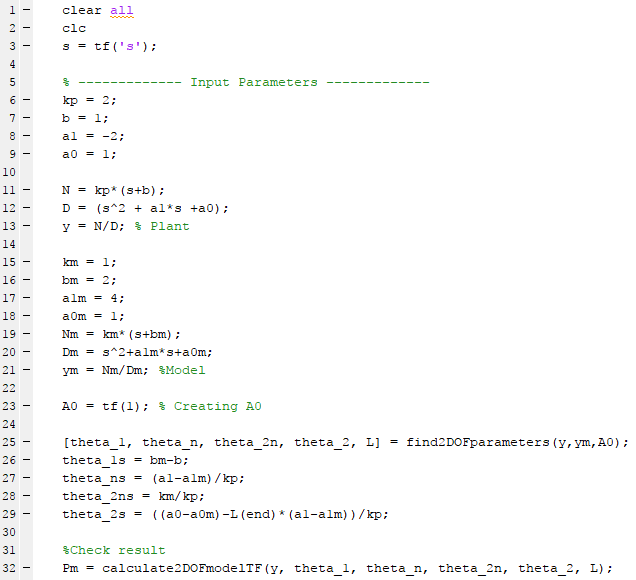
\includegraphics[width=0.8\textwidth]{figs/script1.png}
  \label{fig:script1}
\end{figure}
%
Sa�da da fun��o \textit{calculate2DOFmodelTF.m}:
%
\begin{figure}[H]
  \centering
  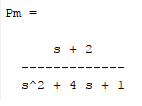
\includegraphics[width=0.2\textwidth]{figs/exemplo1.png}
  \label{fig:exemplo1}
\end{figure}

%---------------------------------------------------------------------
\subsection{Simula��o \#2 ($n = 3, n^{*} = 2$)}

\begin{align*}
  P(s) &= \frac{2s+2}{s^3 +s^2 -2s + 1}\,,  &  P_m(s) &= \frac{1}{s^2 + 4s + 1}\,, & A_0(s) &= s+1 \,,
\end{align*}
%
Script de teste:
%
\begin{figure}[H]
  \centering
  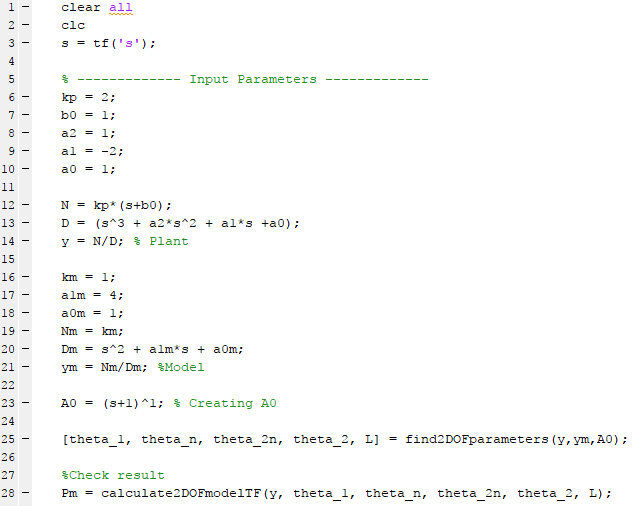
\includegraphics[width=0.8\textwidth]{figs/script2.png}
  \label{fig:script2}
\end{figure}
%
Sa�da da fun��o \textit{calculate2DOFmodelTF.m}:
%
\begin{figure}[H]
  \centering
  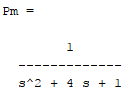
\includegraphics[width=0.2\textwidth]{figs/exemplo2.png}
  \label{fig:exemplo2}
\end{figure}

\newpage
%---------------------------------------------------------------------
\subsection{Simula��o \#3 ($n = 3, n^{*} = 3$)}

\begin{align*}
  P(s) &= \frac{1}{s^3 + s^2 -2s + 1}\,,  &  P_m(s) &= \frac{1}{s^3 +2s^2 + 4s + 1}\,, & A_0(s) &= (s+1)^2 \,,
\end{align*}
%
Script de teste:
%
\begin{figure}[H]
  \centering
  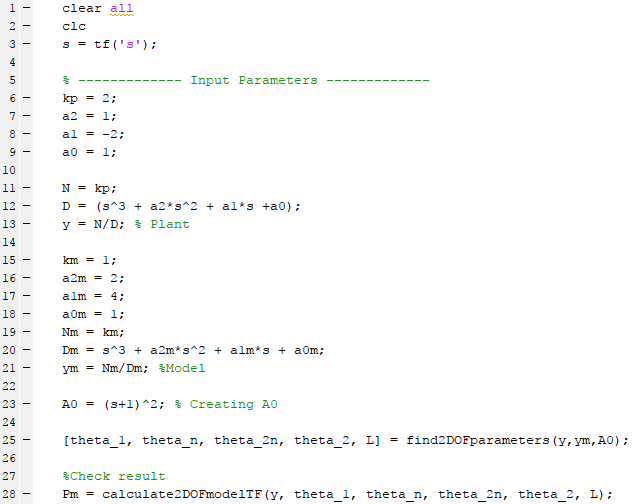
\includegraphics[width=0.8\textwidth]{figs/script3.png}
  \label{fig:script3}
\end{figure}
%
Sa�da da fun��o \textit{calculate2DOFmodelTF.m}:
%
\begin{figure}[H]
  \centering
  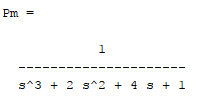
\includegraphics[width=0.25\textwidth]{figs/exemplo3.png}
  \label{fig:exemplo3}
\end{figure}


